\documentclass[10pt,a4paper]{article}
\usepackage[utf8]{inputenc}
\usepackage{amsmath}
\usepackage{amsfonts}
\usepackage{amssymb}
\usepackage{mathtools}
\usepackage{url}

\newcommand{\PDeriv}[2]{\frac{\partial#1}{\partial#2}} % Pour faire des fractions derivees partielle sans trops se casser la tete :) (p. ex. \PDeriv{y(t}{t})
\newcommand{\V}[1]{\overrightarrow{#1}}
\newcommand{\Base}[1]{\widehat{\uline{a_{#1}}}} % Pour les vecteurs de base (MMC) par exemple \Base{1},\Base{2} et \Base{3}

\begin{document}
\title{Projet 4: MS1}
\date\today
\author{Groupe 7}
\maketitle

\section{Trilateration}
	La trilateration est une manière de localiser une cible à partir de trois récepteurs en se basant sur l'estimation du temps de vol entre la cible et un des récepteurs. 
		
		
	Afin de localiser la cible au moins trois récepteurs fixes sont nécessaire. En effet pour chaque récepteur, une fois que le temps de vol est connu, le lieu des points possible pour la position de la cible est un cercle. Entre deux récepteurs ce lieu devient au maximum deux points et avec trois celui-ci est au maximum un point unique. 
		\subsection{Résolution dans le cas idéal}
		Si chaque récepteur se trouve à la position $(x_i , y_i)$ et que sa distance par rapport à l'émetteur est $d_i$ , alors dans un cas idéal, la position de l'émetteur est solution du system \ref{sys}.  
		\begin{equation}
		\begin{dcases}
			(x - x_1)^2 + (y-y_1)^2 = d_1^2 \\
			(x - x_2)^2 + (y-y_2)^2 = d_2^2 \\
			(x - x_3)^2 + (y-y_3)^2 = d_3^2 
		\end{dcases}
		\label{sys}
		\end{equation}
		
		Pour trouver une solution à ce système il est possible de procéder de la manière suivante. Premièrement soustraire deux fois deux équations. Cette soustraction donne une équation de droite qui est donnée par l'équation \ref{eq1} si les équations $i$ et $j$ sont soustraites.
		
		\begin{equation}
			\label{eq1}
			y = \frac{(d_i^2 - d_j^2) - (y_i^2 -y_j^2)-(x_i^2 - x_j^2) + 2x(x_i-x_j)}{-2(y_i-y_j)}
		\end{equation}
		
		L'intersection de deux de ces droites est la solution du système \ref{sys}. 
		
		\subsection{Résolution dans le cas non-idéal}

%\subsection{Résolution dans le cas non-idéal}
Dans le cas non-idéal le système \ref{sys} n'a pas de solution. Il est donc intéressant de chercher une solution approchée. Pour ce faire il faut trouver une expression de l'erreur commise et la minimiser. La distance d'un point $(x_p , y_p)$ à un cercle centrée en $(x_i , y_i)$ et de rayon $d_i$ ( $dist(P , C_i)$) est donnée par l'équation \ref{dist}. L'erreur commise pour une point $P$ est donc la somme de ces distances au carré (equation \ref{err}).
\begin{equation}
dist(P , C_i)= |{\sqrt{(x_i-x_p)^2 +(y_i - y_p)^2} - d_i}|
\label{dist}
\end{equation}

\begin{equation}
\label{err}
err(P) = \sum _{i=1} ^{3} (\sqrt{(x_i-x_p)^2 +(y_i - y_p)^2} - d_i)^2
\end{equation}

Afin de minimiser cette erreur, la méthode itérative de Newton-Raphson est utilisée. Cette méthode consiste en la résolution du système \ref{it} pour chaque pas. Le pas suivant se calcule grâce aux équations \ref{nx} et \ref{ny}. 

\begin{equation}
	\centering
	\begin{pmatrix}
		\frac{\partial^2 f(x_k , y_k)}{\partial x \partial x} & \frac{\partial^2 f(x_k , y_k)}{\partial y \partial x} \\
		\frac{\partial^2 f(x_k , y_k)}{\partial x \partial y} & \frac{\partial^2 f(x_k , y_k)}{\partial y \partial y} 
 	\end{pmatrix} 
 	 \begin{pmatrix}
 	 	\Delta x \\
 	 	\Delta y 
 	 \end{pmatrix}
 	 = - 
 	 \begin{pmatrix}
 	 	\frac{\partial f(x_k , y_k)}{\partial x}\\
 	 	\frac{\partial f(x_k , y_k)}{\partial y} 
 	 \end{pmatrix}
 	 \label{it}
\end{equation}

\begin{equation}
	\centering
	\label{nx}
	x_{k+1} = \Delta x + x_k
\end{equation}


\begin{equation}
	\centering
	\label{ny}
	y_{k+1} = \Delta y + y_k
\end{equation}


			
\section{Multilatération}
On suppose maintenant qu'on n'a plus accès au signal émis (\textit{Tx}) mais qu'on ne dispose que des signaux reçus ($Rx_1$, $Rx_2$ et $Rx_3$), qui nous permettent d'évaluer les différences de temps d'arrivée entre les différents récepteurs ($\tau_{ij}$) la différence de temps d'arrivée entre les récepteurs $i$ et $j$. La différence de distance émetteur-récepteurs vaut alors $d_{ij} = c*\tau_{ij}$, $c$ étant la vitesse de la lumière dans l'air.

\subsection{Lieu des points correspondant}
Le lieu caractérisé par la différence de distance par rapport aux deux récepteurs est une hyperbole. Commençons par traduire la différence de distance. On a $(x,y)$ le point du lieu, $(x_i,y_i)$ et $(x_j,y_j)$ les positions des récepteurs (connues) et $d_{ij}$ la différence de distance. Mathématiquement, ceci se traduit par :

\begin{equation}
\sqrt{(x-x_i)^2 + (y-y_i)^2} - \sqrt{(x-x_j)^2 + (y-y_j)^2} = d_{ij}
\label{Hyperbole}
\end{equation}

On peut ajouter la racine associée à la distance entre $(x,y)$ et $(x_j,y_j)$ aux deux membres puis élever au carré la nouvelle équation. Le reste du développement, assez fastidueux, consiste à ré-arranger les termes obtenus et à ré-élever une nouvelle fois au carré l'équation. Après arrangement des termes, on peut faire apparaître la forme générale d'une conique :

\begin{equation}
Ax^2 + Bxy + Cy^2 + Dx + Ey + F = 0
\end{equation}

avec les constantes suivantes (on définit $\Delta_x = x_i - x_j$, $\Delta_y = y_i - y_j$ et $k = (x_i^2 - x_j^2) + (y_i^2 - y_j^2) - d_{ij}^2$ pour alléger les notations) :


$$\begin{cases}
A = 4(\Delta_x^2 - d_{ij}^2)\\
B = 8\Delta_x \Delta_y\\
C = 4(\Delta_y^2 - d_{ij}^2)\\
D = 4(2d_{ij}^2x_j-k\Delta_x)\\
E = 4(2d_{ij}^2y_j-k\Delta_y)\\
F = k^2-4d_{ij}^2(x_j^2+y_j^2)\\
\end{cases}$$

On sait que le signe du discriminant $B^2 - 4AC$ détermine le type de conique. Ici, ce discriminant est proportionnel à :

\begin{equation}
det = B^2 - 4AC \propto (\Delta_x^2 + \Delta_y^2) - d_{ij}^2 = \mathrm{dist}(i,j)^2 - d_{ij}^2\geq 0
\end{equation}

La dernière inégalité s'interpète comme suit : la différence des distances récepteur-source est plus petite que la distance entre les deux recepteurs (notée $\mathrm{dist}(i,j)$), ce qui est assez trivial avec un peu d'intuition géométrique. Formulons toutefois une démonstration rigoureuse : on se place dans le triange formé par les deux récepteurs et l'émetteur. On a $d_i$/$d_j$ la distance entre l'émetteur et le récepteur $i$/$j$ ($d_{ij} = d_i - d_j$), et toujours $\mathrm{dist}(i,j)$ la distance entre les récepteurs. On sait que la somme de deux côtés du triangle est plus grande que le dernier côté :

\begin{equation}
\mathrm{dist}(i,j) + d_j \geq d_i \Rightarrow \mathrm{dist}(i,j) \geq d_i - d_j = d_{ij}
\end{equation}

Ce qui permet d'écrire la dernière inégalité du discriminant. Le lieu est donc bien une hyperbole\footnote{Sauf un cas particulier : celui ou on a $d_{ij} = \mathrm{dist}(i,j)$. Cette dégénérescence apparait quand l'émetteur est situé sur la droite formée par les deux récepteurs (mais ne se situe pas entre eux).} car le déterminant de la conique est positif.

\subsection{Nombre de mesures nécessaires.}
On dispose de trois différence de distance ($d_{12}$, $d_{23}$ et $d_{31}$, les autres ne donnent bien évidemment pas d'indications supplémentaires car il s'agit des mesures "opposées" à celles déjà mentionnées). Est-ce assez?

Deux coniques quelconques ne peuvent avoir que 4 intersection au maximum (sans être les mêmes)\footnote{source : \url{http://ocw.upm.es/algebra/affine-and-projective-geometry/contenido/apuntes_ocw/week12_ocw.pdf}}. 

Deux mesures laissent donc, dans le pire cas, quatre locations possibles. On pourrait penser qu'une mesure additionnelle pourrait, par manque de chance, ne pas apporter assez d'informations et passer par les quatre points déjà candidats ; ceci est toutefois impossible. Il suffit de se dire que les trois foyers (les trois récepteurs) forment les trois sommets d'un triangle (du moins si on les a disposés ainsi) et d'un peu d'intuition géométrique pour s'en convaincre. En fait, il y aura toujours deux intersections restantes. Soit deux solution possibles.

Parfois, le signe des $d_{ij}$\footnote{Le signe nous indique les récepteur se trouve le plus proche de la cible et donc quelle moitié de l'hyperbole est à considérer} permet de sauver la mise. Mais, parfois, comme idiqué figure \ref{int}, il n'est pas possible sur base des mesures uniquement de distinguer les deux solutions. Trois mesures ne sont donc parfois pas suffisantes, ce qui pourrait expliquer certaines erreurs de localisation par la suite. Un quatrième récepteur permettrait d'éliminer toute ambiguïté concernant la localisation de l'émetteur.

\begin{figure}[h]
\centering
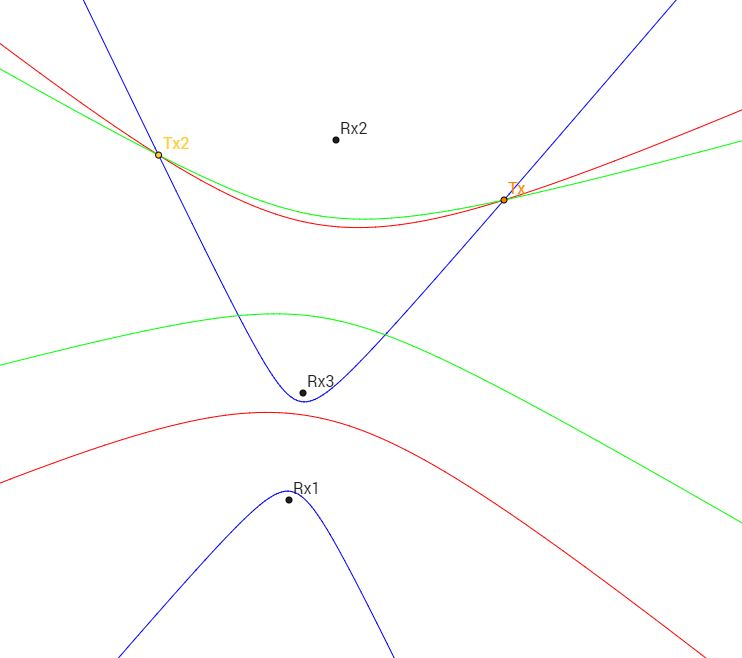
\includegraphics[scale = 0.5]{hyperbole}
\caption{Deux intersections possibles de 3 hyperboles. Malgré ce que le graphique pourrait laisser deviner, les trois récepteurs sont non-collinéaires.}
\label{int}
\end{figure}

\subsection{Résolution pratique}
Comme en réalité les intersections ne sont pas parfaites, on ne peut pas résoudre directement les équations. On va donc trouver une autre voie, pour traiter les erreurs sur les $d_{ij}$.

On définit ainsi le résidu $r_{ij}$ associé à chaque $d_{ij}$ : 

\begin{equation}
r_{ij}(x,y) = \sqrt{(x-x_i)^2 + (y-y_i)^2} - \sqrt{(x-x_j)^2 + (y-y_j)^2} - d_{ij}
\end{equation}

Le résidu est nul si le point se situe sur l'hyperbole. Le résidu mesure donc en quelque sorte donc la distance entre l'hyperbole et le point associé à l'émetteur. On va minimiser la somme de la valeur absolue des résidus :

\begin{equation}
\mathrm{min}_{(x,y)} | r_{12}(x,y)| + |r_{23} (x,y)| + |r_{31} (x,y)|
\end{equation}

En pratique, il a fallu filtrer les signaux reçus pour éliminer un maximum de bruit, sans quoi les estimations des temps d'arrivées étaient complètement faussées. Deux filtres de Butterworth ont été utilisés.

Il y a encore deux types d'erreur. Premièrement, les filtres ne sont pas encore assez performants et les estimations de position ne sont pas toujours fiables à cause du bruit. Il y a un deuxième souci avec le programme actuel car même en prenant les valeurs "excactes" des différences de temps d'arrivée (enfin, en utilisant le signal émis pour les calculer plus facilement, ce qui est "tricher") on tombe, pour le troisième jeu de données, à côté de l'émetteur. Cette erreur pourrait être due à une autre intersection des trois hyperboles (voir plus haut), mais son origine excacte n'a pas encore été identifée.

Les figures \ref{ex1} à \ref{ex3} sont des exemples de figures obtenues avec le code actuel. Dans les meilleurs cas, l'erreur est de moins d'un mètre, mais parfois l'effet du bruit dans la corrélation donne des résultats farfelus (une location à plus de $70m$ de l'objectif, pas de graphe car pas très intéressant). Il y a aussi le problème du troisième jeu de données, déjà mentionné, non identifié.

\begin{figure}[h]
\centering
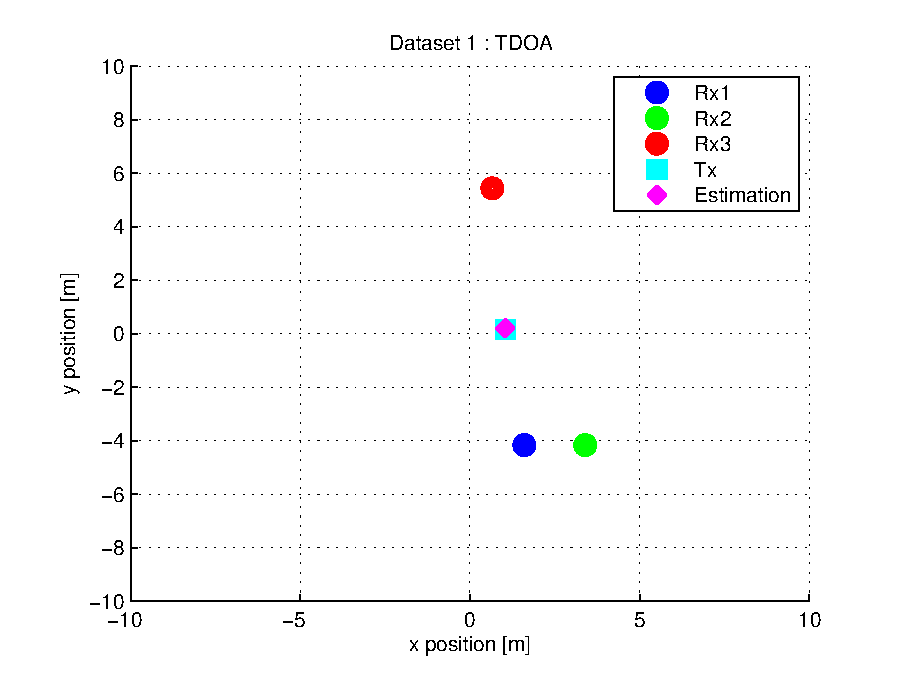
\includegraphics[scale = 0.5]{TDOA1}
\caption{Jeu de données 1. Ici, les différences de temps sont correctement estimées et la position est presque exacte.}
\label{ex1}
\end{figure}

\begin{figure}[h]
\centering
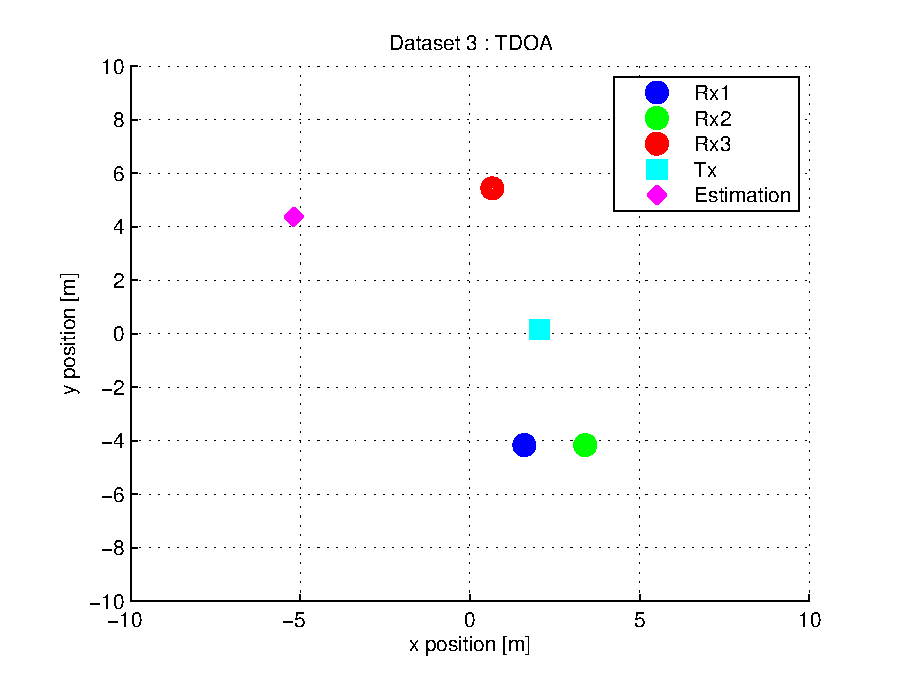
\includegraphics[scale = 0.5]{TDOA3}
\caption{Jeu de données 3. Les estimations de différence de temps sont les mêmes que celles obtenues en utilisant $Tx$, mais on tombe très loin de la cible.}
\label{ex2}
\end{figure}

\begin{figure}[h]
\centering
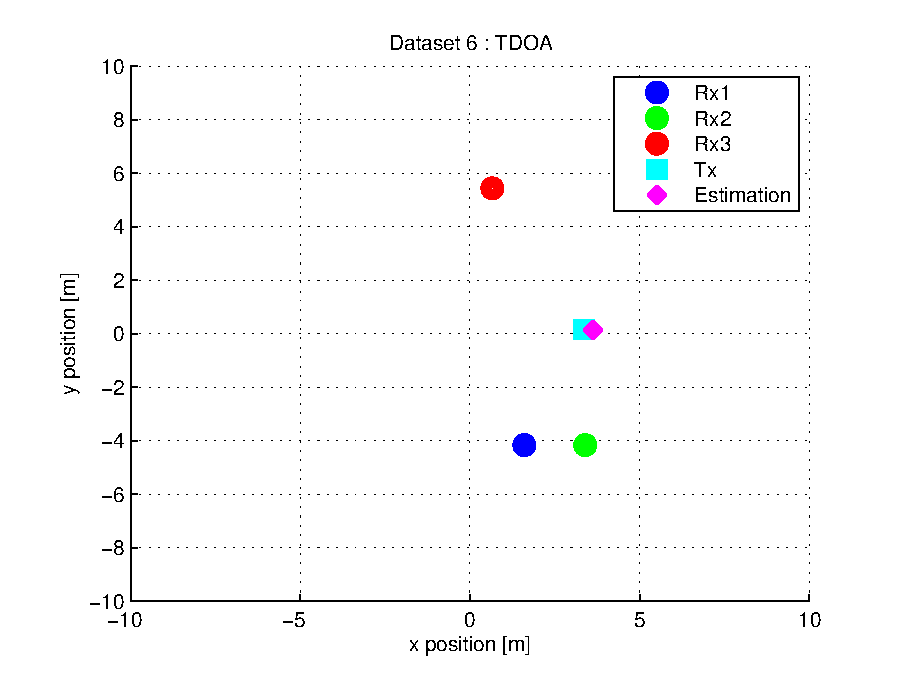
\includegraphics[scale = 0.5]{TDOA6}
\caption{Jeu de données 6.}
\label{ex3}
\end{figure}


\section{Échantillonnage}
On a affaire à deux signaux $s(t)$ et $r(t)$ qui sont tout deux situés dans la bande de fréquence de 6GHz à 8GHz. On va s'intéresser à l'échantillonnage de tels signaux.
\begin{figure}[h!]
\centering
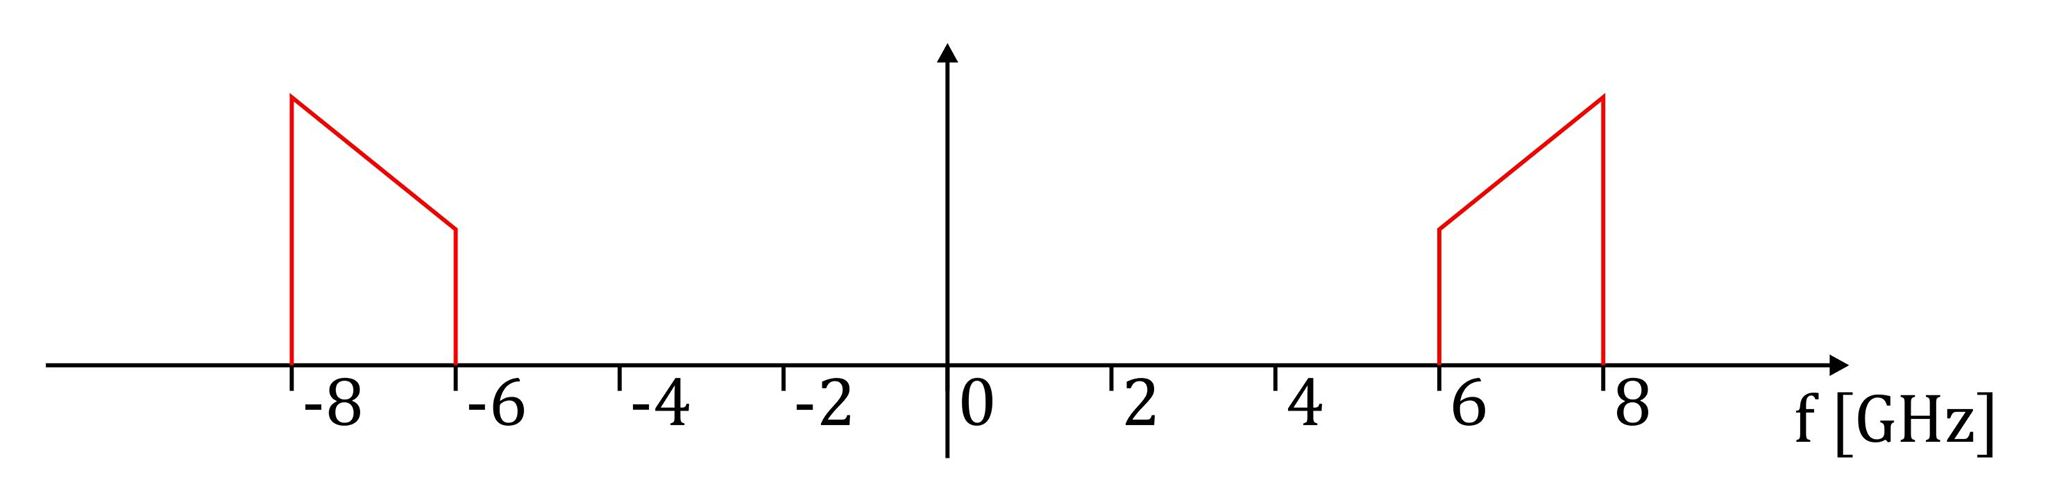
\includegraphics[scale=0.2]{sig.jpg}
\caption{signal de base dans le domaine fréquentiel}
\label{sig}
\end{figure}
\subsection{Théorème de Nyquist}
Afin d'être sûr de ne pas avoir affaire à un repli spectral, il est suffisant de respecter le théorème d'échantillonnage de Shannon-Nyquist\footnote{condition suffisante mais pas nécessaire comme il sera démontré plus loin}. Ce théorème donne la condition suivante: $f_e\geqslant 2f_{max}$ dans notre cas, la fréquence d'échantillonnage minimale est donc: $f_e=16\text{GHz}$.
\subsection{Échantillonnage du signal donné}
On peut maintenant échantillonner le signal donné à la figure \ref{sig}. Regardons ce qu'il en est pour une fréquence d'échantillonnage $f_e$ de 4GHz. Lorsqu'un signal en temporel est discret, cela impose que le signal dans le domaine fréquentiel est périodique avec une fréquence de répétition égale à $f_e$. On obtient donc le signal de la figure \ref{sig2}. Il est intéressant de remarquer qu'on ne respecte pas la condition de Nyquist mais qu'on a tout de même évité un repli spectral qui déteriorerait le signal. Il est donc possible, à priori, de récupérer le signal originel malgré la "faible" fréquence d'échantillonnage.
\begin{figure}[h!]
\centering
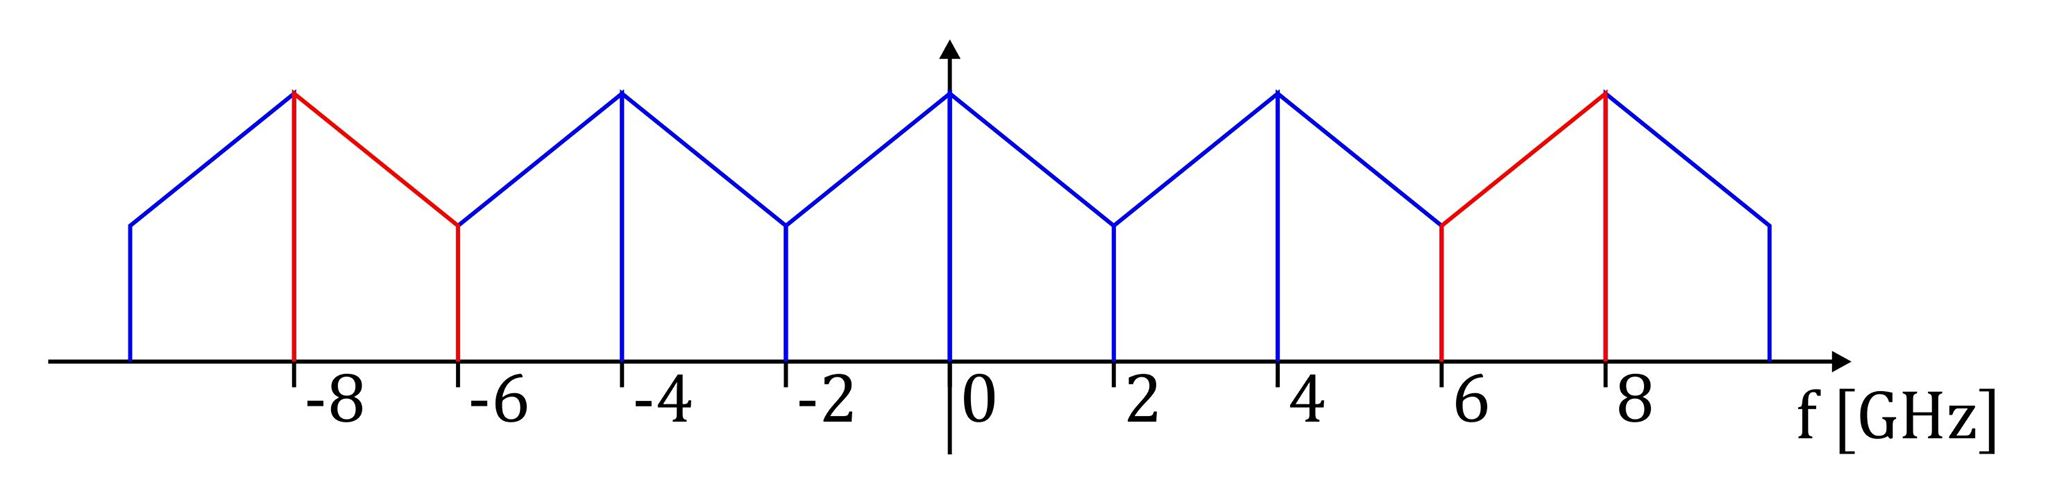
\includegraphics[scale=0.2]{sig2.jpg}
\caption{signal échantillonné dans le domaine fréquentiel}
\label{sig2}
\end{figure}
\subsection{Signal échantillonné}
Regardons maintenant l'expression du signal $r(t)$ lorsqu'il est échantillonné à la fréquence $f_e$. On défini ce signal discret comme $r[n]$.\\
On sait qu'échantillonner revient à multiplié le signal continu $r(t)$ par un train de deltas de Dirac espacés de la période d'échantillonnage $T_e=1/f_e$. On obtient donc:
$$r[n]=r(t)\sum_{n=-\infty}^{\infty}\delta (t-nT_e)$$
Ce qui revient à dire:
$$r[n]=\sum_{n=-\infty}^{\infty}r(nT_e)\delta (t-nT_e)$$
\subsection{Récupération du signal de départ}
On veut maintenant retrouver le signal de départ $r(t)$ à partir du signal échantillonné $r[n]$. On peut voire sur la figure \ref{sig2} que le signal de départ de la figure \ref{sig} peut être obtenu grâce à un filtre passe-bande allant de 6GHz à 8GHz. Cela n'est possible que parce qu'il n'y a pas eu de recouvrement dans le domaine fréquentiel lors de l'échantillonnage. On aurait pas pu récupérer notre signal avec $f_e=2\text{GHz}$ par exemple.\\
On va donc multiplier le signal de la figure \ref{sig2} par le signal en domaine fréquentiel suivant:
$$ H(j\omega )=\left\{ 
\begin{tabular}{cc}
1 & 2$\pi .6$ GHz $< | \omega | <$ 2$\pi .8$ GHz \\ 
0 & \text{ailleurs} \\ 
\end{tabular} 
\right. $$
On a donc un produit dans le domaine fréquentiel ce qui correspond à un produit de convolution dans le domaine temporel.
$$R(j\omega )\cdot H(j\omega )\Longleftrightarrow \left(\sum_{n=-\infty}^{\infty}r[n]\delta (t-nT_e)\right)\ast h(t)$$
Avec $h(t)=\text{TFI}(H(j \omega ))$. On peut donc faire le développement suivant en posant $a=2\pi .6$ GHz et $b=2\pi .8$ GHz:
\begin{eqnarray*}
h(t) & = &\frac{1}{2\pi}\int_{-\infty}^{\infty}H(j\omega )\cdot \exp^{j\omega t}d\omega \\
& = & \frac{1}{2\pi}\int_{a}^{b}1\cdot \exp^{j\omega t}d\omega + \frac{1}{2\pi}\int_{-b}^{-a}1\cdot \exp^{j\omega t}d\omega\\
& = & \frac{1}{2\pi j t}\left[ \exp^{j\omega t}\right]_a^b - \frac{1}{2\pi j t}\left[ \exp^{j\omega t}\right]_{-a}^{-b}
\end{eqnarray*}
Or on peut poser $a=\omega_m-\omega_0$ et $b=\omega_m+\omega_0$ avec dans notre cas $\omega_m=7\text{GHz}$ et $\omega_0=1\text{GHz}$. Cela donne:
\begin{eqnarray*}
h(t) & = &\frac{1}{2\pi j t}\left[ \exp^{j\omega t}\right]_{\omega_m-\omega_0}^{\omega_m+\omega_0} - \frac{1}{2\pi j t}\left[ \exp^{j\omega t}\right]_{-\omega_m+\omega_0}^{-\omega_m-\omega_0}\\
& = & \exp^{j\omega_m t}\frac{\sin (\omega_0 t)}{\pi t} + \exp^{-j\omega_m t}\frac{\sin (\omega_0 t)}{\pi t}
\end{eqnarray*}
Ce résultat est satisfaisant vu qu'on observe bien la présence de deux exponentielles complexes dépendant de $\omega_m$. Cela vient du décalage de la fenêtre de largeur $2\omega_0$ de $\pm \omega_m$ dans le domaine fréquentiel.\\
Il suffit maintenant d'effectuer le produit de convolution avec le signal discret:
\begin{equation}
r(t)=\left(\sum_{n=-\infty}^{\infty}r[n]\delta (t-nT_e)\right)\ast \left( \exp^{j\omega_m t}\frac{\sin (\omega_0 t)}{\pi t} + \exp^{-j\omega_m t}\frac{\sin (\omega_0 t)}{\pi t} \right)
\end{equation}

\end{document}
